\section{Iterative Method} \label{section:iter}
In the first approach, we actually execute each query multiple times with different configuration parameters to determine the optimal set of parameters. For each candidate set of configuration parameters, the query is run and the target metric, such as total resource usage, is measured. By comparing the metrics across different runs with different configuration parameters, we can determine a good set of parameters to use. 

\subsection{Assumptions}
\label{sec:assumptions}
\begin{figure*}[h]
	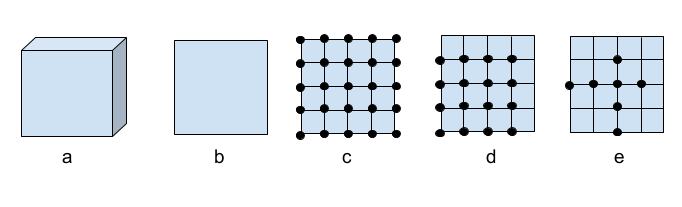
\includegraphics[width=\linewidth]{fig/searchspace.png}
	%\vspace*{-15pt}
	\caption{Reducing the search space}
	\label{fig:searchspace}
\end{figure*}


The main challenge in such methods is to limit the number of trials, since each execution takes up resources and has a monetory cost associated with it. Earlier approaches based on iterative execution have used various techniques such as noisy gradient~\cite{KumarPLPGB16} to converge to a solution faster. In our method, we make use of domain knowledge and heuristics to reduce the search space. Specifically, we employed the following strategies to reduce the parameter space to be explored.

\noindent\subsubsection*{\bf Parameter reduction: }
\label{sec:paramreduction}
The search space is exponential in the number of parameters to be optimized. There are a large number of parameters that can be set for any query. As described in Section~\ref{sec:optmethod}, we have identified a smaller set of parameters that have a relatively larger impact on the performance of sql queries. We restrict the search to these parameters, thus reducing the search space. These parameters have been listed in Tables~\ref{table:job_params}. The search space with a restricted set of parameters is shown in Figure~\ref{fig:searchspace}(b).
\noindent\subsubsection*{\bf Discretization: }
Each parameter, such as memory or partition size, can take a large number of values. However, it can be observed that small changes in the parameters do not have a significant impact. Thus, instead of trying each possible value, it is sufficient to discretize the parameter range and consider only a subset of values for each parameter. These values are placed at a reasonable distance from each other so as to have a significant impact on the query performance. For example, instead of varying memory in units of 1 MB, we can vary it in multiples of 128 MB. The resulting search space is shown in Figure~\ref{fig:searchspace}(c).
\noindent\subsubsection*{\bf Range reduction: }
The range of values for each parameter is further restricted based on domain knowledge about what a good range for that parameter would be.  The knowledge about a good range can be gained by either talking to experts or by looking at some other metrics. For example, for the Hive on MR engine, consider the mapper\_time metric that measures the average time taken by a mapper. If the mapper time is too low, the overhead of starting the mappers is large compared to the actual work done by the mapper. Since the mapper time is inversely related to the number of mappers, the number of mappers need to be reduced. On the other hand, if the mapper time is large, then the job parallelism is restricted and the end to end clock time taken for the query will be high. In this case, more mappers are needed to reduce the work that each mapper has to do. A good acceptable range for this metric could be from 240s till 1800s.  If a set of config params results in mapper\_time beyond the acceptable range, it should not be considered in the search process. For example, mapper\_time is affected by mapreduce.input.fileinputformat.split.maxsize and the correlation is direct, i.e. mapper\_time  increases as we increase mapreduce.input.fileinputformat.split.maxsize.  Thus the split maxsize should be constrained to a range that will lead to a reasonable mapper\_time. In our experiments, we restricted splitsize to between 128 MB and 1 GB. The resulting search space is shown in Figure~\ref{fig:searchspace}(d).
\noindent\subsubsection*{\bf Dimension independence: } 
We make an assumption that the parameters are not correlated to each other. This enables us to optimize each parameter independently of the others. Thus, rather than exploring all the points in the search space, the algorithm explores only one set of values for each parameter as shown in Figure~\ref{fig:searchspace}(e). This is a very strong assumption, which may not hold in practice. For example, the mapper memory (mapreduce.map.memory.mb) and the splitsize (mapreduce.input.fileinputformat.split.maxsize) are correlated, since more memory is needed by the mappers as the splitsize increases if spills are to be avoided. Even in this case, the algorithm will find the best value for memory after fixing the splitsize or the best splitsize after fixing the memory. So overall the configuration chosen will be a reasonably good one.

\subsection{Algorithm}
The overall method is listed in Algorithm~\ref{alg:iterativesearch} and is fairly straightforward. It starts with the default value for each configuration parameter (Line 1). It then iterates over the parameters and for each parameter it explores a range of values from low to high, varying it with a minimum step size (Lines 2--6). It runs the query with the chosen parameter values and measures the metric (such as running time or utilization). It finds the value for which the metric is optimized and fixes the value of the parameter to that value before moving on the next parameter (lines 7--12). Finally, it outputs the set of good parameter values $V$ that are discovered in the process.
\renewcommand{\algorithmicrequire}{\textbf{Input:}}
\renewcommand{\algorithmicensure}{\textbf{Output:}}
\renewcommand{\algorithmiccomment}[1]{// #1}
\begin{algorithm}[h]
	\caption{\bf \textit{Iterative Search}}
	\label{alg:iterativesearch}
	\begin{algorithmic}[1]
		%\vspace{1.3em}
		%\small
		\footnotesize
		\REQUIRE Set $\mathcal{P}$ = $\{p_1, p_2 \ldots p_n\}$ of parameters to be determined, the metric $m$ to be optimized, the query $Q$
		\ENSURE The values for parameters in $\mathcal{P}$ that optimize $m$
		\STATE Let $V$ = $\{v_1, v_2, \ldots v_n\}$ = $\{p_1^d, p_2^d, \ldots p_n^d\}$
		\COMMENT {$p_i^l$, $p_i^d$, $p_i^h$ and $p_i^s$ denote the low value, default value, high value and discrete step size for parameter $p_i$}		
		\FOR {Param $p_i$ in $\mathcal{P}$}
			\STATE $m_{best} \gets null$
			\FOR {Value $v$ from $p_i^l$ to $p_i^h$ in steps of $p_i^s$} 
				\STATE Replace $v_i$ by $v$ in $V$
				\STATE Run $Q$ with parameter setting $V$ and measure the metric $m$
				\IF {$m_{best}$ is $null$ or $m$ is better than $m_{best}$}
					\STATE $m_{best} \gets m$
					\STATE $v_{best} \gets v$
				\ENDIF
			\ENDFOR
			\STATE Replace $v_i$ by $v_{best}$ in $V$ \COMMENT{Best value for parameter $p_i$ is found and used in further search}			
		\ENDFOR
		\RETURN $V$
    \end{algorithmic}
\end{algorithm}
  
\subsection{Results}
We evaluated the effectiveness and practicality of the iterative method by running experiments on both synthetic and real workloads. The experiments were carried out for a Hive on MR engine. The results demonstrated the importance of optimizing the configuration parameters, but at the same time motivated us to explore the model based method instead of the iterative method. We thus present the results here before moving on to describing the model based approach.

\subsubsection*{Synthetic Workload}
For synthetic workload, we used the TPC DS dataset (scale 1000) and queries. Each query had to be run a number of times to discover a good set of configuration parameters. To keep the time for the experiments reasonable, we had to use a somewhat small dataset. The average data read by each query was of the order of 20 to 40 GB. The experiments were run on a 4 node cluster on AWS with machine type r3.xlarge. The metric to be optimized was the total resource utilization (Equation~\ref{eqn:totalresource}) and parameters whose values are to be determined are the ones mentioned earlier in Table~\ref{table:job_params}. For each query, we compare the best and worst configuration discovered with the default one in terms of the resource utilization. The results are shown in Figure~\ref{fig:iterativetpcds}. It plots the ratios of the resource usage of minimum to default, maximum to default and maximum to minimum. The min corresponds to the best configuration discovered and max corresponds to the worst configuration among the ones tried out. The graph shows that the min to default ratio varies from 0.18 to 0.73, which indicates that the iterative search leads to a configuration that can save upto 82\% in resource usage over the default configuration. The ratio of max to default is mostly close to 1 and in some cases goes upto 1.80. This indicates that in many cases, the default configuration itself was the worst one (same as max). This is due to the fact that the default split size was 128 MB, leading to a large number of mappers, each processing small amount of data. Since there is some overhead (5-10s) in starting the JVM for each mapper, the startup time becomes significant percentage of the total mapper time if the mapper itself takes very less time to process the data. As a result, the overall query time suffers and resource utilization increases. This suggests that a different default with a larger split size would be more appropriate. Finally, the ratio of max to the min varies from 1.47 to 5.41, indicating that the configuration parameters do make a significant difference in query execution. 
\begin{figure}[h]
	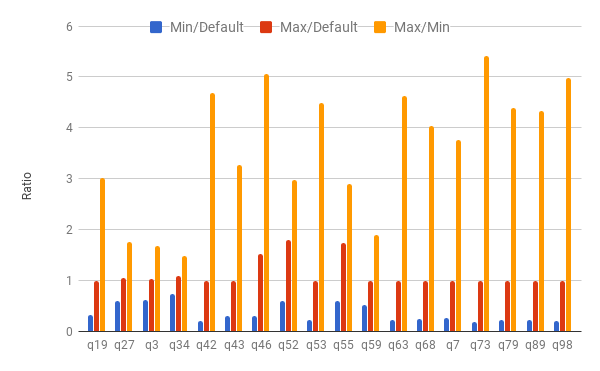
\includegraphics[width=\linewidth]{fig/tpcds-iterative.png}
	%\vspace*{-15pt}
	\caption{Iterative algorithm on TPC DS\protect\footnotemark[1]}
	\label{fig:iterativetpcds}
\end{figure}

\subsubsection*{Real Workloads}
We evaluated the iterative method over real customer data and queries (Customer 1). The workload consisted of three Hive queries running on Hadoop2 MR. These queries were very large and complex and part of their analytics workflow. The input data size was about 400 GB for two of the queries and 200 GB for the third query. The cluster consisted of a r3.2xlarge master node and 30 slave nodes of type r3.8xlarge on AWS Cloud. Figure~\ref{fig:iterativelyft} shows the percentage savings in the total resource utilization cost (Equation~\ref{eqn:totalresource}) of the three queries with the configuration discovered by the iterative algorithm, compared to the cost with the configuration that the customer was using in production. The results show that the iterative algorithm was able to achieve significant savings upto 77\% even for production workloads, indicating that many production workloads are not fully optimized. However, the iterative algorithm took over 50 hours and cost \$5000 since the cluster was quite large with expensive machines. 
\begin{figure}[h]
	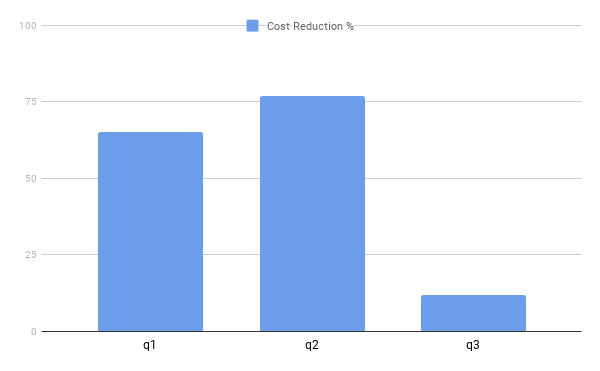
\includegraphics[width=\linewidth]{fig/lyft.png}
	%\vspace*{-15pt}
	\caption{Iterative algorithm on real workload}
	\label{fig:iterativelyft}
\end{figure}

\subsubsection*{Discussion}
The results on synthetic and real datasets show that finding good configuration parameters can lead to significant savings in query costs. The iterative algorithm is able to discover good configuration parameters in a small number of iterations (usually around 10-15 iterations). However, there are some practical limitations as listed below:
\begin{itemize}
	\item The dollar cost of the optimization process can be significant as seen in the real workload. In this case, the customer had 1000 more queries. It may be possible to make the search more efficient and reduce the number of iterations. Since  customers have 100s or 1000s of queries, even 10 or 50 fold reduction is not sufficient to make the approach economical.
	\item For ETL queries, the approach requires shadow clusters and queries. The queries had to be reviewed multiple times to make sure production clusters and tables were not affected. The cost in terms of man-hours is also exorbitant. 	
\end{itemize} 
To address these concerns, we propose a cost model based optimization approach next that does not require multiple executions of the query with different parameters.
